

\tikzset{every picture/.style={line width=0.75pt}} %set default line width to 0.75pt        

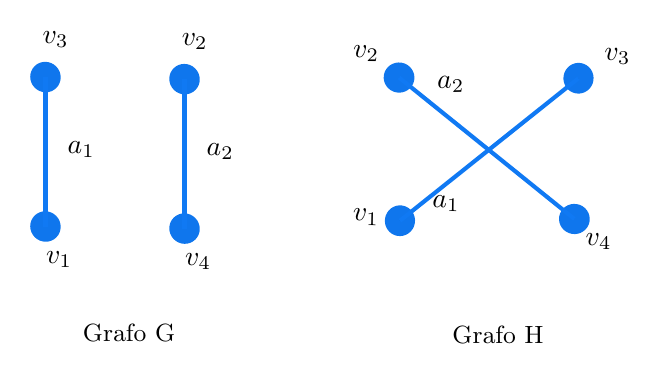
\begin{tikzpicture}[x=0.75pt,y=0.75pt,yscale=-1,xscale=1]
%uncomment if require: \path (0,173); %set diagram left start at 0, and has height of 173

%Shape: Ellipse [id:dp7672867321663941] 
\draw  [draw opacity=0][fill={rgb, 255:red, 15; green, 118; blue, 237 }  ,fill opacity=1 ] (20.6,20.43) .. controls (23.46,17.61) and (28.1,17.68) .. (30.98,20.59) .. controls (33.85,23.5) and (33.87,28.15) .. (31.01,30.97) .. controls (28.16,33.79) and (23.51,33.72) .. (20.63,30.8) .. controls (17.76,27.89) and (17.74,23.25) .. (20.6,20.43) -- cycle ;
%Shape: Ellipse [id:dp7060944758385839] 
\draw  [draw opacity=0][fill={rgb, 255:red, 15; green, 118; blue, 237 }  ,fill opacity=1 ] (20.6,92.43) .. controls (23.46,89.61) and (28.1,89.68) .. (30.98,92.59) .. controls (33.85,95.5) and (33.87,100.15) .. (31.01,102.97) .. controls (28.16,105.79) and (23.51,105.72) .. (20.63,102.8) .. controls (17.76,99.89) and (17.74,95.25) .. (20.6,92.43) -- cycle ;
%Straight Lines [id:da6791312533711067] 
\draw [color={rgb, 255:red, 16; green, 121; blue, 243 }  ,draw opacity=1 ][fill={rgb, 255:red, 0; green, 0; blue, 0 }  ,fill opacity=1 ][line width=1.5]    (25.81,25.7) -- (25.81,97.7) ;
%Shape: Ellipse [id:dp7766028650957342] 
\draw  [draw opacity=0][fill={rgb, 255:red, 15; green, 118; blue, 237 }  ,fill opacity=1 ] (87.6,21.43) .. controls (90.46,18.61) and (95.1,18.68) .. (97.98,21.59) .. controls (100.85,24.5) and (100.87,29.15) .. (98.01,31.97) .. controls (95.16,34.79) and (90.51,34.72) .. (87.63,31.8) .. controls (84.76,28.89) and (84.74,24.25) .. (87.6,21.43) -- cycle ;
%Shape: Ellipse [id:dp13385211505551253] 
\draw  [draw opacity=0][fill={rgb, 255:red, 15; green, 118; blue, 237 }  ,fill opacity=1 ] (87.6,93.43) .. controls (90.46,90.61) and (95.1,90.68) .. (97.98,93.59) .. controls (100.85,96.5) and (100.87,101.15) .. (98.01,103.97) .. controls (95.16,106.79) and (90.51,106.72) .. (87.63,103.8) .. controls (84.76,100.89) and (84.74,96.25) .. (87.6,93.43) -- cycle ;
%Straight Lines [id:da7874419899288638] 
\draw [color={rgb, 255:red, 16; green, 121; blue, 243 }  ,draw opacity=1 ][fill={rgb, 255:red, 0; green, 0; blue, 0 }  ,fill opacity=1 ][line width=1.5]    (92.81,26.7) -- (92.81,98.7) ;
%Shape: Ellipse [id:dp3478384831309793] 
\draw  [draw opacity=0][fill={rgb, 255:red, 15; green, 118; blue, 237 }  ,fill opacity=1 ] (188.85,24.75) .. controls (189.5,20.79) and (193.29,18.11) .. (197.33,18.76) .. controls (201.37,19.42) and (204.12,23.16) .. (203.48,27.12) .. controls (202.84,31.08) and (199.04,33.76) .. (195,33.11) .. controls (190.97,32.45) and (188.21,28.71) .. (188.85,24.75) -- cycle ;
%Shape: Ellipse [id:dp6943800404481995] 
\draw  [draw opacity=0][fill={rgb, 255:red, 15; green, 118; blue, 237 }  ,fill opacity=1 ] (273.33,92.89) .. controls (273.97,88.92) and (277.77,86.24) .. (281.8,86.9) .. controls (285.84,87.55) and (288.6,91.3) .. (287.95,95.26) .. controls (287.31,99.22) and (283.52,101.9) .. (279.48,101.25) .. controls (275.44,100.59) and (272.69,96.85) .. (273.33,92.89) -- cycle ;
%Straight Lines [id:da30491395610387206] 
\draw [color={rgb, 255:red, 16; green, 121; blue, 243 }  ,draw opacity=1 ][fill={rgb, 255:red, 0; green, 0; blue, 0 }  ,fill opacity=1 ][line width=1.5]    (196.17,25.93) -- (280.64,94.07) ;
%Shape: Ellipse [id:dp22454624869229134] 
\draw  [draw opacity=0][fill={rgb, 255:red, 15; green, 118; blue, 237 }  ,fill opacity=1 ] (283.78,18.95) .. controls (287.75,19.58) and (290.44,23.37) .. (289.79,27.41) .. controls (289.15,31.45) and (285.42,34.21) .. (281.45,33.58) .. controls (277.49,32.95) and (274.8,29.16) .. (275.44,25.12) .. controls (276.08,21.08) and (279.82,18.32) .. (283.78,18.95) -- cycle ;
%Shape: Ellipse [id:dp2585636244259957] 
\draw  [draw opacity=0][fill={rgb, 255:red, 15; green, 118; blue, 237 }  ,fill opacity=1 ] (197.77,87.59) .. controls (201.73,88.22) and (204.43,92.01) .. (203.78,96.05) .. controls (203.14,100.09) and (199.41,102.86) .. (195.44,102.23) .. controls (191.48,101.6) and (188.78,97.81) .. (189.43,93.77) .. controls (190.07,89.73) and (193.8,86.96) .. (197.77,87.59) -- cycle ;
%Straight Lines [id:da09856693560407126] 
\draw [color={rgb, 255:red, 16; green, 121; blue, 243 }  ,draw opacity=1 ][fill={rgb, 255:red, 0; green, 0; blue, 0 }  ,fill opacity=1 ][line width=1.5]    (282.62,26.26) -- (196.61,94.91) ;

% Text Node
\draw (23,2.4) node [anchor=north west][inner sep=0.75pt]    {$v_{3}$};
% Text Node
\draw (24.63,108.2) node [anchor=north west][inner sep=0.75pt]    {$v_{1}$};
% Text Node
\draw (35,55.4) node [anchor=north west][inner sep=0.75pt]    {$a_{1}$};
% Text Node
\draw (90,3.4) node [anchor=north west][inner sep=0.75pt]    {$v_{2}$};
% Text Node
\draw (91.63,109.2) node [anchor=north west][inner sep=0.75pt]    {$v_{4}$};
% Text Node
\draw (102,56.4) node [anchor=north west][inner sep=0.75pt]    {$a_{2}$};
% Text Node
\draw (293.55,10.54) node [anchor=north west][inner sep=0.75pt]  [rotate=-358.99]  {$v_{3}$};
% Text Node
\draw (172.63,87.65) node [anchor=north west][inner sep=0.75pt]  [rotate=-1.25]  {$v_{1}$};
% Text Node
\draw (210.87,81.28) node [anchor=north west][inner sep=0.75pt]  [rotate=-0.73]  {$a_{1}$};
% Text Node
\draw (172.63,9.07) node [anchor=north west][inner sep=0.75pt]  [rotate=-0.52]  {$v_{2}$};
% Text Node
\draw (284.63,99.48) node [anchor=north west][inner sep=0.75pt]  [rotate=-0.16]  {$v_{4}$};
% Text Node
\draw (212.96,24.01) node [anchor=north west][inner sep=0.75pt]  [rotate=-358.65]  {$a_{2}$};
% Text Node
\draw (42.39,143.44) node [anchor=north west][inner sep=0.75pt]  [font=\small] [align=left] {Grafo G};
% Text Node
\draw (220.39,144.44) node [anchor=north west][inner sep=0.75pt]  [font=\small] [align=left] {Grafo H};


\end{tikzpicture}